\documentclass[11pt]{article}
\usepackage[margin = 0.5in]{geometry}
\usepackage[utf8]{inputenc}
\usepackage{blindtext}
\usepackage{graphicx}
\usepackage{multirow}
\usepackage{subfig}
\graphicspath{ {./images/} }


\begin{document}

\title{MiniProject 2}
\author{
    Seyed Yazdan Zinati
    \and
    SeyedBehnam Mashari
    \and
    Mohammadhadi Foroutan
}

\maketitle

\begin{abstract}
    In this project, we studied the performance of linear classification models, namely multinomial naive Bayes and logistic regression on two textual datasets for binary and multiclass classification. Although the logistic regression model outperformed multinomial naive Bayes on the IMDb dataset in terms of accuracy by 5\% (87\% vs 82\%), both models achieved similar accuracies when applied on the 20newsgroup dataset with about 70\%. Notwithstanding, it is worth mentioning that the naive Bayes model is computationally more expensive than the logistic regression model, making logistic regression faster and more energy-efficient classifier. We used 5-fold cross-validation to tune the hyperparameters of our models on both datasets to achieve the best performance. We compared the models implemented from scratch to Scikit learn models where applicable. For instance, our logistic regression model showed better accuracy for binary classification on the IMDb dataset than the Scikit-learn model.

    Furthermore, we explored the impact of using subsets of training data and features on the accuracy of our models. We observed only slight changes in the models' accuracy as a smaller set of features was utilised. However, while decreasing the number of features improved the models' performance on the IMDb dataset, it somewhat decreased the performance on the 20newsgroup dataset. We found that the performance of the models on the 20newsgroup dataset depended more heavily on the amount of information they were trained on compared to the IMDb dataset. For instance, while enlarging the size of data the models were trained on increased the accuracy on both datasets, this gain in accuracy was more significant on the 20newgroup dataset. These findings are consistent with the results in [2]. To further evaluate our models, performance metrics such as the ROC curve and confusion matrix were studied.
\end{abstract}

\section{Introduction}
Although information is available in many forms, text is probably the largest repository of human knowledge. Nevertheless, analyzing huge amounts of unstructured text data from emails, social media conversations, chats, and reviews is extremely challenging. Not only manually processing an enormous amount of text data is time-consuming, but it is expensive, error-prone, and tedious. Text analysis can have a range of methods and techniques including text classification, clustering, word sentence disambiguation, to name but a few. Text classification itself has a wide range of applications in sentiment analysis, intent detection and topic modelling.

In this domain, preprocessing techniques are required for converting these documents to structured documents [1]. Before converting raw textual data to numerical data, we followed some steps to clean and preprocess the datasets effectively. We worked with the bag-of-words model which is a simplifying representation in natural language processing commonly used in methods of document classification where the occurrence of words are used as features for training a classifier.

Linear classification models are used for multiclass and binary classifications. Identifying the weight of a word in a text and how much is the existence importance of that word in the text is evaluated by the number of times that word is seen in the text. TF-IDF is a statistical measure enabling us to scale the weight of a word in the text. It was demonstrated in [3] that using TF-IDF scores instead of raw word frequencies improved the performance of multinomial naive Bayes.

In this work, we utilized multinomial naive Bayes and linear regression models. We concluded that the linear regression model is more accurate in performing binary classification on the IMDb reviews dataset whereas, multinomial naive Bayes outperforms logistic regression for multiclass classification on the 20newsgroup dataset. It is noteworthy that rather than using other naive Bayes methods such as Gaussian naive Bayes and Bernoulli naive Bayes, we used multinomial naive Bayes, a logarithm based classifier, which is more suitable for the classification of textual data [2, 4]. The results of implemented models on the IMDb reviews dataset are comparable with outcomes in [5].

\section{Datasets}
Two datasets are subjects of analysis in this project: “Twenty Newsgroups text dataset” and “Large movie IMDB review dataset”.  Twenty Newsgroups is a standard dataset fetched from the sklearn library, containing 18846 samples (posts) and 20 classes (different newsgroups). This dataset is divided into 11314 training and 7532 testing samples. The IMDb review dataset encompasses 50k samples in which the training set and testing set are equally split. The training set is divided into positive and negative reviews, in other words, binary sentiment polarity labels where a negative review has a rating smaller or equal to 4 out of 10, a positive review has a rating greater or equal to 7 out of 10 and reviews with more neutral ratings are not included.

To better understand the datasets, we visualized class distributions, most common n-grams, word clouds, etc. For example, positive and negative IMDb reviews word clouds are illustrated in Figure 1 (a) and (b). Additional dataset visualizations can be found in the submitted Notebook.


\begin{figure}[h]
    \centering
    \subfloat[\centering Postive reviews]{{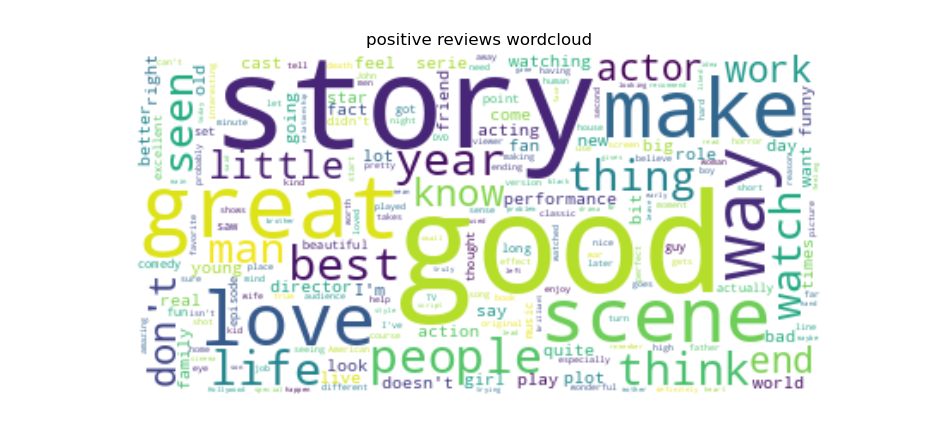
\includegraphics[width=7.8cm]{Fig7} }}%
    \quad
    \subfloat[\centering Negative reviews]{{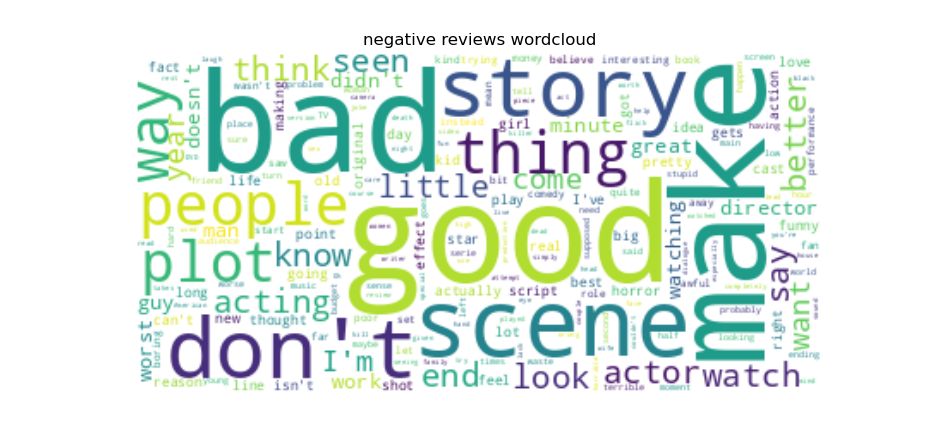
\includegraphics[width=7.8cm]{Fig8} }}%
    \label{fig:wordcloud}%
    \caption{IMDb reviews sentiment wordclouds}%
\end{figure}
To begin the preprocessing stage, the 20newsgroup dataset is loaded from Scikit-learn while the IMDb dataset was constructed from raw text files. The constructed IMDb reviews dataset was then saved to be loaded on the next program runs due to this process being time-consuming. In this step, we assure that both datasets are in a similar format, enabling us to feed them into the same preprocessing subroutine. The 20newsdataset is cleaned from headers, footers and quotes. Furthermore, we replace all punctuations and delimiters such as tabs,  endlines, and carriage returns with space delimiters.

After this initial cleaning step, we analyzed the most frequent words appearing in datasets, as shown in Figure 2(a). Despite the frequent use of these words in natural language, a large number of them give us no or low value information in training our models. These words referred to as stop words  (such as "the", "and", "of", and to") are filtered out of our training data. Other measures taken in this step to further filter out trivial information from our training set include lower casing all characters as well as removing accents, numbers, special characters. Figure 2(b) depicts the most frequent words appearing in the IMDb reviews dataset after taking the mentioned steps.
\begin{figure}[h]
    \centering
    \subfloat[\centering]{{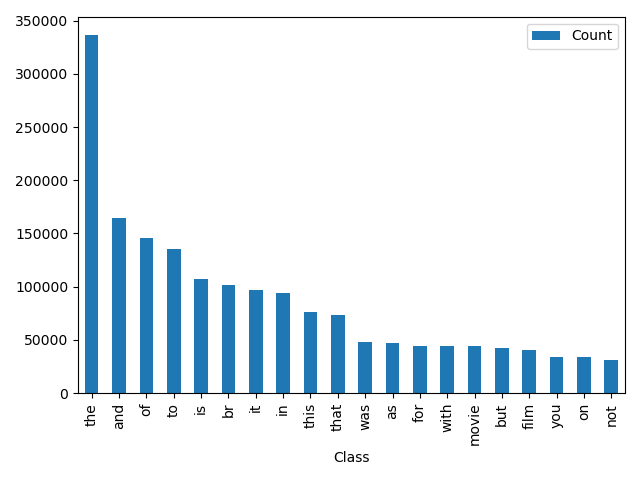
\includegraphics[height=4.95cm]{Fig1} }}%
    \quad
    \subfloat[\centering]{{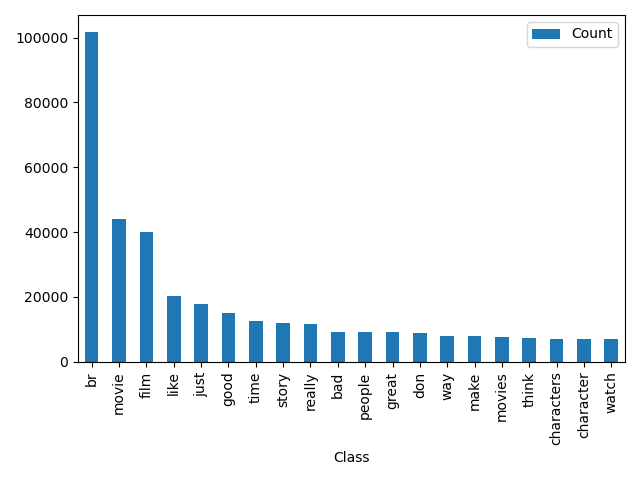
\includegraphics[height=4.96cm]{Fig2} }}%
    \label{fig:wordcloud}%
    \caption{IMDb reviews dataset before (a) and after (b) feature engineering and removing stopwords}%
\end{figure}

Taking a closer look at Figure 2(b), it can be observed that the word "character" and "characters" are considered to be distinct. However, both of these words give us the same information. This is only a good case in point. A solution to this problem would be stemming or lemmatization, as words with one stem (family word) need to be reduced to a common base form. Stemming chops off the ends of words, whereas lemmatization determines the base of the word. Among these techniques, we use lemmatization as a more reliable way to reduce inflectional and derivationally related forms of a word. To verify this claim, we compared accuracies by deploying both techniques using the natural language toolkit (NLTK) which resulted in a better outcome for lemmatization.

Once the raw text files have been feature engineered, cleaned, and lemmatized, they need to be transformed in the form of feature vectors to be appropriate for statistical analysis. The bag of words method is used to generate vectors containing the occurrences of each word in documents. After obtaining word frequencies in each document, those which occur numerous times in many samples are considered less informative. For this reason, we downscale those frequencies using the TF-IDF statistical measure. Using this method, in turn, lessens the influence of repetitive less informative words. Since each document contains only a few words, there will be many zeros in our matrix. Using a dense matrix will be extremely memory expensive, as our matrix contains a large number of zeros, we input sparse matrices to our models for training.

\section{Results}
Two classification models particularly multinomial naive Bayes and logistic regression are applied to both datasets. We wrote the multinomial naive Bayes and logistic regression models from scratch, able to perform multiclass and binary classification respectively. To tune the hyperparameters of our models, we performed 5-fold cross-validation using our implementation. The hyperparameter for multinomial naive Bayes is alpha, the smoothing factor. Learning rate, maximum iterations, and the inverse of regularization strength constitute our hyperparameters for Logistic regression. Due to the cross-validation being time-consuming, we used a randomized search as an alternative to an exhaustive search in some cases. The alpha leading to the highest accuracy using multinomial naive Bayes was found to be equal to 0.01 and 0.61 for the 20newsgroup , and IMDb reviews dataset correspondingly.  As for logistic regression, a learning rate of 10, a max iteration of 320, and an inverse of regularization strength of 10 achieved the highest accuracy for both datasets. We then evaluated the performance of our models using accuracy and weighted F1 score stated in Table 1. F1 score is an appropriate measure used to balance Precision and Recall when there is an uneven class distribution.

\begin{table}
    \caption {Comparison of the two classification models on both datasets}
    \centering
    \begin{tabular}{|l|l|l|l|l|}
        \hline
        Model                                    & Dataset      & Accuracy & F1 Score~ & 5-fold cv accuracy  \\
        \hline
        \multirow{2}{*}{Multinomial naive Bayes} & IMDb review  & 0.82684 & 0.82721    & 0.86564                    \\
        \cline{2-5}
                                                 & 20newsgroup  &    0.70074     & 0.70643          & 0.76710                     \\
                                                 \hline
        \multirow{2}{*}{Logistic regression}     & IMDb reviews &     0.8742     &  0.87420         &         0.89160            \\
        \cline{2-5}
                                                 & 20newsgroup  &   0.69078       &  0.69027         & 0.75455                    \\
                                                 \hline
    \end{tabular}
\end{table}

\section{Discussion and Conclusion}

\section{Statement of Contribution}

\newpage
% add references here
\end{document}
